%\newtheorem{definition}{Definition}
\newtheorem{lemma}{Lemma}
\newtheorem{theorem}{Theorem}
\newtheorem{proposition}{Proposition}
\newtheorem{corollary}{Corollary}
\newtheorem{conjecture}{Conjecture}
%\newtheorem{claim}{Claim}
%\newtheorem{property}{Property}
\newtheorem{example}{Example}

% Marius commands
\newcommand{\Z}{{\mathbb Z}}
\newcommand{\N}{{\mathbb N}}
\newcommand{\relmat}[1] { \{\!\!\{#1\}\!\!\}}
\newcommand{\matrel}[1] { [\!\![#1]\!\!]}
\newcommand{\key}[1]{\underline{#1}}

% semantic stuff
\newcommand{\bi}[1]{{}^\omega\!{#1}^\omega}
\newcommand{\rbr}{{\bf ]\!]}}
\newcommand{\lbr}{{\bf [\![}}
\newcommand{\sem}[1]{\lbr #1 \rbr}
\newcommand{\model}[2]{\sem{#1}_{#2}}
\newcommand{\lfp}[1]{\mbox{fix}\ {#1}}
\newcommand{\wpr}{\widetilde{pre}}
\newcommand{\cceil}[1]{\lfloor #1 \rfloor + 1}

\renewcommand{\vec}[1]{{\bf {#1}}}

% alias
\newcommand{\alias}{\Diamond}
\newcommand{\may}[2]{{\langle #1 \rangle}{#2}}
\newcommand{\must}[2]{{\lbrack #1 \rbrack}{#2}}
\newcommand{\defd}[1]{\delta({#1})}

% logic
\newcommand{\pal}{$pAL$}
\newcommand{\wal}{$wAL$}
\newcommand{\kal}{$\kappa AL$}

% cardinal, degree, ...
\newcommand{\sgn}{\mbox{sgn}}
%\newcommand{\gcd}{\mbox{gcd}}
\newcommand{\lcm}{\mbox{lcm}}
\newcommand{\len}[1]{{|{#1}|}}
\newcommand{\card}[1]{{|\!|{#1}|\!|}}
\newcommand{\minimum}[2]{\mbox{min}({#1},{#2})}
\newcommand{\maximum}[2]{\mbox{max}({#1},{#2})}
\newcommand{\minset}[2]{\mbox{min}\{{#1}\ |\ {#2}\}}
\newcommand{\maxset}[2]{\mbox{max}\{{#1}\ |\ {#2}\}}
\newcommand{\divs}[1]{\mbox{div}({#1})}

% automata and languages
\newcommand{\auth}[1]{{\mathcal A}_{#1}}
\newcommand{\lang}[1]{{\mathcal L}({#1})}
\newcommand{\runs}[1]{{\mathcal R}({#1})}
\newcommand{\val}[1]{{\mathcal V}({#1})}
\newcommand{\trace}[1]{{Tr}({#1})}
\newcommand{\state}[1]{{\Sigma}({#1})}
\newcommand{\trans}[1]{{\Theta}({#1})}
\newcommand{\access}[3]{{\mathcal L}_{{#1},{#2}}({#3})}
\newcommand{\eats}{\rightarrow}
\newcommand{\Eats}[1]{\stackrel{#1}{\longrightarrow}}
\newcommand{\arrow}[2]{\xrightarrow[{\scriptstyle #2}]{{\scriptstyle #1}}}
\newcommand{\larrow}[2]{\xleftarrow[{\scriptstyle #2}]{{\scriptstyle #1}}} 

% numbers
\newcommand{\nat}{{\bf \mathbb{N}}}
\newcommand{\zed}{{\bf \mathbb{Z}}}
\newcommand{\bool}{{\bf \mathbb{B}}}
\newcommand{\rat}{{\bf \mathbb{Q}}}
\newcommand{\real}{{\bf \mathbb{R}}}
\newcommand{\linzed}{{\bf \mathcal{L}\mathbb{Z}}}

% powerset
\newcommand{\pow}[1]{{\mathcal P}(#1)}
\newcommand{\pown}[2]{{\mathcal P}^{#1}(#2)}

% by definition
\newcommand{\bydef}{\stackrel{\Delta}{=}}

% projection, lifting
\newcommand{\proj}[2]{{#1}\!\!\downarrow_{{#2}}}
\newcommand{\lift}[2]{{#1}\!\!\uparrow_{{#2}}}

% forward, backward
\newcommand{\forw}[1]{\stackrel{\rightarrow}{#1}}
\newcommand{\back}[1]{\stackrel{\leftarrow}{#1}}

% equation figures
\newcommand{\eqnfigx}[1]{
\begin{minipage}{3in}
\begin{center}
\begin{eqnarray*}#1
\end{eqnarray*}
\end{center}
\end{minipage}}

\newcommand{\twoeqnfigx}[2]{
\eqnfigx{#1}
\eqnfigx{#2}
}

\newcommand{\threeeqnfigx}[3]{
\eqnfigx{#1}\\
\eqnfigx{#2}\eqnfigx{#3}
}

\newcommand{\eqnfig}[1]{
\begin{minipage}{3in}
\begin{center}
\begin{eqnarray}#1
\end{eqnarray}
\end{center}
\end{minipage}}

\newcommand{\twoeqnfig}[2]{
\eqnfig{#1}
\eqnfig{#2}
}

% transitions and SOS rules
\newcommand{\storetrans}[1]{\stackrel{#1}{\leadsto}}
\newcommand{\storetransx}[1]{\stackrel{#1}{\leadsto^*}}
\newcommand{\storetransprime}[3]{{#1} \storetrans{#2} {#3}}
\newcommand{\gammatrans}[1]{\stackrel{#1}{\hookrightarrow}}
\newcommand{\gammatransprime}[3]{{#1} \gammatrans{#2} {#3}}
\newcommand{\gammatransx}[1]{\stackrel{#1}{\hookrightarrow^*}}
%\newcommand{\trans}[3]{{#1} \stackrel{#2}{\longrightarrow} {#3}}
\newcommand{\run}[3]{{#1} \stackrel{#2}{\Longrightarrow} {#3}}
\newcommand{\sosrule}[2]{\frac{\begin{array}{c}#1\end{array}}{#2}}
\newcommand{\hoare}[3]{\{#1\}\ {\bf #2}\ \{#3\}}

\newcommand{\derivone}[3]{\mbox{\infer[#3]{#2}{#1}}}
\newcommand{\derivtwo}[4]{\mbox{\infer[#4]{#3}{{#1} & {#2}}}}
\newcommand{\derivdot}[4]{\mbox{\infer[#4]{#3}
{\begin{array}{l} {#1} \\ \vdots \\ {#2} \end{array}}}}

% comments, paragraphs
\newcommand{\comment}[1]{\vspace{\baselineskip}\noindent\fbox{
\parbox[b][\height][s]{120mm}{#1}}}
\newcommand{\mypar}[1]{\vspace*{\baselineskip}\noindent\emph{#1}}

% theories
\newcommand{\arith}{\langle \zed, +, \cdot, 0, 1 \rangle}
\newcommand{\hilbert}{\langle \zed, +, \cdot, 0, 1 \rangle^\exists}
\newcommand{\presbg}{\langle \zed, \geq, +, 0, 1 \rangle}
\newcommand{\divides}{\langle \zed, +, |, 0, 1 \rangle}
\newcommand{\lipshitz}{\langle \zed, \geq, +, |, 0, 1 \rangle^\exists}
\newcommand{\dioph}[1]{\mathfrak{D}(#1)}

% proofs
\newif\ifLongVersion\LongVersionfalse
%\newcommand{\proof}[1]{\noindent {\em Proof}: {#1}}
%\renewcommand{\qed}{$\Box$\vspace*{\baselineskip}}
%\newcommand{\qed}{$\Box$\vspace*{\baselineskip}}
\newcommand{\inproof}[1]{\ifLongVersion \proof{#1} \fi}
%\newcommand{\outproof}[2]{\ifLongVersion \else \vspace*{\baselineskip}\noindent Proof of {#1}: \proof{#2} \fi}


\documentclass[compress]{beamer}
%\documentclass{beamer}

\usepackage{beamerthemeJuanLesPins}
\usepackage{amsfonts,amsmath,amsthm,amssymb}
\usepackage{graphicx}
\usepackage{epsfig}
\usepackage{listings}

\usepackage[latin1]{inputenc}
%\usepackage{dcpic,pictex} %for commutative diagrams

\newcommand\xor{\oplus}
\newcommand{\emath}[1]{\ensuremath{#1}}
  \newcommand\tred[1]{\textcolor{red}{#1}}
  \newcommand\tblue[1]{\textcolor{blue}{#1}}
\newcommand\tgreen[1]{\textcolor{green}{#1}}
%\newcommand\tred[1]{\textcolor{red}{#1}}
%\usepackage[small,nhug,heads=vee]{diagrams}
%\diagramstyle[labelstyle=\scriptstyle]

\newcommand{\gspace}[0]{\hspace{2mm}}

\newcommand{\gnt}[1]{\langle \textit{#1} \rangle}
\newcommand{\gntsp}[1]{\gnt{#1} \gspace}
\newcommand{\gntm}[1]{$\gnt{#1}$}

\newcommand{\bbb}[1]{\mathbf{#1}}

\newcommand{\ga}[0]{::=}
\newcommand{\gam}[0]{$\ga$}

%\newcommand{\glit}[1]{\textrm{'}{\texttt{#1}}\textrm{'}}
%\newcommand{\glit}[1]{{\textbf{'}\textbf{#1}\textbf{'}}}
\newcommand{\glit}[1]{{\textbf{#1}}}
\newcommand{\glitsp}[1]{\glit{#1} \gspace}
\newcommand{\glitm}[1]{$\glit{#1}$}

\newcommand{\lparc}[0]{\textbf{'$\{$'}}
\newcommand{\rparc}[0]{\textbf{'$\}$'}}
\newcommand{\lparcsp}[0]{\lparc \gspace}
\newcommand{\rparcsp}[0]{\rparc \gspace}

\newcommand{\garrow}[0]{\textbf{'}\texttt{->}\textbf{'}}
\newcommand{\garrowsp}[0]{\garrow \gspace}

\newcommand{\gor}[0]{\\ & | &}
\newcommand{\gornb}[0]{\gspace | \gspace} % no break

\newcommand{\gsec}[1]{\noindent\textbf{#1}}

\newcommand{\spaceaptr}[0]{\hspace{1mm}}





%%%%%%%%%%%%%%%%%%%%%%  SSL RELATED STUFFS %%%%%%%%%%%%%%%%%%%%%%%%%%
%%%%%%%%%%%%%%%%%%%%%%%%%%%%%%%%%%%%%%%%%%%%%%%%%%%%%%%%%%%%%%%%%%%%%

\newcommand{\bi}[1]{{}^\omega\!{#1}^\omega}
\newcommand{\rbr}{{\bf ]\!]}}
\newcommand{\lbr}{{\bf [\![}}


\newcommand{\sem}[1]{\lbr #1 \rbr}

\newcommand{\arrow}[2]{\xrightarrow[{\scriptstyle #2}]{{\scriptstyle #1}}}

\newcommand{\defeq}[0]{:=}
\newcommand{\syntaxeq}[0]{::=}

\newcommand{\Dom}[1]{\mathcal{D}om(#1)}

\newcommand{\rrule}[2]{\lstinline!#1!  \to \lstinline!#2!}
\newcommand\Addr{\mathcal{A}ddr} %The set of heap addresses
\newcommand\LVar{\mathcal{L}Var} %The set of location variables
\newcommand\PVar{\mathcal{P}Var} %The set of pointer variables.

\newcommand{\Pp}[1]{PP(#1)} %% The set of the atomic propositions that appear inside a formula.
\newcommand{\Sp}[1]{SP(#1)} %% The set of spacial propositions that appear insde a formula.


%Size of a formula.
\newcommand{\sizef}[1]{|{#1}|}
%subformula
\newcommand{\subf}[0]{\triangleright}

\newcommand{\gton}[1]{>_{#1}}
\newcommand{\gtlvar}[0]{\gton{\LVar}}
\newcommand{\gtptrvar}[0]{\gton{\PVar}}

\newcommand{\Locvar}[1]{Locvar(#1)} %The set of location variables appearing
	%in a formula
\newcommand{\Ptrvar}[1]{Ptrvar(#1)} %same as abovem but for Ptr variables.

\newcommand{\NULL}[0]{\mbox{\texttt{NULL}}}

\newcommand{\Alloc}[1]{alloc(#1)}
\newcommand{\Emp}{\lstinline{Emp}}

\newcommand{\Unsep}[0]{\ast}
\newcommand{\Sep}[2]{#1 \Unsep #2}
\newcommand{\Sepf}[2]{ #1 \star #2}

\newcommand{\EqLoc}[2]{ (#1 = #2) }
\newcommand{\Andpure}[2]{ #1 \wedge #2}
\newcommand{\Pointsto}[2]{ #1 \mapsto #2}
\newcommand{\nil}[0]{\lstinline!nil!}
\newcommand{\Pointstonil}[1]{ #1 \mapsto \mbox{\nil}}
\newcommand{\Formula}[2]{ #1  \updownarrow #2}
\newcommand{\Exists}[2]{ \exists #1. #2}

\newcommand{\Substin}[3]{#1\lbrack #2 \gets #3 \rbrack}
\newcommand{\NForm}[1]{\mathcal{NF}(#1)}

\newcommand{\Ran}[1]{\mathcal{R}an(#1)}

\newcommand{\Vars}[1]{\mathcal{V}ars(#1)}
\newcommand{\FVars}[1]{\mathcal{F}Vars(#1)}


\newcommand{\Equa}[1]{\mathcal{E}q(#1)}
\newcommand{\Aff}[1]{\mathcal{A}ff{#1}}
\newcommand{\Nullptr}[1]{\mathcal{N}ullptr{#1}}


\newcommand{\Subst}[3]{#3\lbrack #1\leftarrow #2 \rbrack}
\newcommand{\fundec}[5]{\begin{array}{llll} {#1}:&{#2} &\mapsto & {#3} \\ &{#4} & \mapsto& #5  \end{array}}


% add/replaces A.P. #2 in formula #1.
\newcommand{\Addrep}[2]{#1 \lbrack #2 \rbrack}


%%%%%%%%%%% Compute new name for existential variables %%%%%%%%

\newcommand{\renfresh}[2]{Renfresh(#1,#2)}



%%%%%%%%%% Order Relation %%%%%%%%%%%%%%%%%%%%%%%%%%%
\newcommand{\LocOrderIneq}[0]{\sqsubset_{I}}
\newcommand{\LocOrderIeq}[0]{\sqsubseteq_{I}}
\newcommand{\PtrOrderIneq}[0]{\sqsubset_{S}}
\newcommand{\PtrOrderIeq}[0]{\sqsubseteq_{S}}
\newcommand{\ModOrderIeq}[0]{\sqsubseteq_{I,S}}
\newcommand{\ModOrderIneq}[0]{\sqsubset_{I,S}}


\newcommand{\true}{true}
\newcommand{\false}{false}
\newcommand{\dk}{dk}
%% #1 var name, #2 base, size, #4 offset
\newcommand{\ptrexp}[3]{\left ( \begin{array}{l} 
\ptrbase{#1}=#2 \\ 
\ptroffset{#1}=#3
\end{array} \right )}


\newcommand{\base}[2]{base_{#1}(#2)}
\newcommand{\samebase}[3]{Same\_base_{#1}({#2},{#3})}

\newcommand{\lbase}[1]{#1_{base}}
\newcommand{\lsize}[1]{#1_{size}}

\newcommand{\locvar}[3]{
\left ( \begin{array}{l}
\lbase{#1}=#2 \\
\lsize{#1}=#3
\end{array} \right )
}
%%%%%%%%%%%%% Hoar triples and sematic transformations %%%%%%%%%%%%%%%%%

%     instr  
% {P} -----> {Q}
%     effect
\newcommand{\transmodel}[4]{\lbrace #1 \rbrace \arrow{#2}{#3} \lbrace #4 \rbrace }

\newcommand{\Pre}[0]{\lbrace P \rbrace}
\newcommand{\Post}[0]{\lbrace Q \rbrace}

%%%%%%%%%%%% Footprint related stuff %%%%%%%%%%%%%%%%%%%%%%%%%%%%


%%%%%%%%%%%%%%%%%%%%%%%%%%%%%%%%%%%%%%%%%%%%%%%%%%%%%%%%%%%%%%



\newcommand{\ptrbase}[1]{{#1}_{base}}
\newcommand{\ptrsize}[1]{{#1}_{size}}
\newcommand{\ptroffset}[1]{{#1}_{off}}
\newcommand{\gmallocid}[0]{mid}


\newcommand{\interpretZ}[1]{\sem{#1}_{\mathbb{Z}}}
\newcommand{\interpretI}[1]{\sem{#1}_{I}}
\newcommand{\interpretP}[1]{\sem{#1}_{P}}
\newcommand{\interpretC}[1]{\sem{#1}_{C}}

\newcommand{\Eval}[1]{Eval(#1)}

%%%%%%%%%%%%%%%%%%% Validity interpretation compters 
\newcommand{\ival}[1]{{#1}_{\mbox{valid}}}

%%%%%%%%%%%%%%%%%%%%%%%%%%%%%%%%%%%%%%%%%%%%%%%%%%%%%%%%%%%%%%%%%%%%
% Inline text typology and other short notation definitions        %

\newcommand{\nth}[1]{$#1^{\mbox{th}}$}
\newcommand{\rd}[1]{$#1^{\mbox{rd}}$}


\newcommand{\syneq}[0]{::=} %Syntatic definition
\newcommand{\seq}[0]{\equiv} %Syntactic equality/equivalence

%%%%%%%%% Arithmetic operations
\newcommand{\intval}[2]{\left ( \begin{array}{l} #1 \\ #2 \end{array} \right )}

\newcommand{\valid}[1]{{#1}_{\mbox{\lstinline!valid!}}}
\newcommand{\intptr}[2]{\left ( \begin{array}{l} {#1} \\ {#2} 

\end{array} \right )}

\newcommand{\segfault}[0]{\mbox{\lstinline!segfault!}}

\newcommand{\andmath}[0]{\mbox{and}}
\newcommand{\congmod}[3]{#1 \equiv #2 \lbrack #3 \rbrack}
\newcommand{\notcongmod}[3]{#1 \not\equiv #2 \lbrack #3 \rbrack}
\newcommand{\isvalid}[2]{Valid_{#1}(#2)}
\newcommand{\DK}[2]{DK_{#1}(#2)}
%\newcommand{\interpa}[2]{Tr_{#1}(#2)}
\newcommand{\interpa}[2]{\sem{#2}_{#1}}

\newcommand{\interpacomp}[2]{Comp_{#1}(#2)}
\newcommand{\FRAMAC}{FRAMA-C}
\newcommand{\sizeof}[1]{\mbox{\lstinline!sizeof!}(#1)}

%% Counter associated to an interger variable.
\newcommand{\icnt}[1]{#1_{\mbox{cnt}}}

%% Access to memory @ pointer address P :
\newcommand{\accs}[1]{\mbox{\lstinline!access!}(#1)}

\newcommand{\clisting}[1]{\begin{lstlisting}[language=C,basicstyle=\ttfamily,keywordstyle=\color{red}] {#1} \end{lstlisting}}

%%%%%%%%%%%%%%%%%% SSL RELATED STUFFS END BLOCK %%%%%%%%%%%%%%%%%%%%
%%%%%%%%%%%%%%%%%%%%%%%%%%%%%%%%%%%%%%%%%%%%%%%%%%%%%%%%%%%%%%%%%%%%  
  
  

%  \newcommand\bo[1]{\mathcal{#1}}
%  \newcommand\mA{\bo{A}}
%  \newcommand\terminemachin{+a.s. }
%  \newcommand\truc\terminemachin
%  \newtheorem{proposition}{Proposition}
%  \newtheorem{condition}{Condition}
%  \newtheorem{exemple}{Exemple}
%  \newtheorem{theoreme}{Theor�me}
%
%  \newtheorem{notation}{Notation}
%  \newcommand\notat[2]{\begin{condition}[#1] #2 \end{condition}}
%
%  \newcommand\cond[2]{\begin{condition}[#1] #2 \end{condition}}
%  \newtheorem{remarque}{Remarque}
  \usepackage{latexsym}
  \usepackage{graphicx}

%\input{../macros}


%\defbeamertemplate*{section page}{default}[1][]
%{
%  \centering
%    \begin{beamercolorbox}[sep=8pt,center,#1]{section title}
%      \usebeamerfont{section title}\insertsection\par
%    \end{beamercolorbox}
%}
%\newcommand*{\sectionpage}{\usebeamertemplate*{section page}}









  \title{The Flata-C Verification Font End}
 % \part{Main}


%  \author{Radu Iosif, Florent Garnier}
\author{Florent Garnier}
\begin{document}
\frame{\titlepage 
}

\date{April 2013}
%\part{Main}


%\begin{frame}
%\frametitle{Outline}
% \tableofcontents[section,pausesections]
%\end{frame}

\part{Introducing myself}
\frame{\partpage}

\section{ Curriculum :}
\frame{
\frametitle{About Florent Garnier}
\begin{block}{Education}
\begin{itemize}
\item Ph.D. in computer Sciences; Institut National Polytechique de Lorraine, INRIA-Lorraine. 
 \begin{itemize}
   \item Proving the Termination of rules based randomized systems. 
   \item Modeling distributed randomized protocols and proving
     they satisfy liveness properties.
   \item Term rewriting
 \end{itemize}
\item M.D. in Mathematics and Computer Sciences; Universit\'e de Versailles SQY.
 \begin{itemize}
 \item Stochastic processes
 \item Formal Calculus
 \item Graph Theory and Graph algorithmic
 \end{itemize}
\end{itemize}
\end{block}
}

\frame{
\frametitle{Recent Activities}
\begin{block}{Recent activites}
\begin{itemize}
\item Reseach concerning C programs analysis and verification techniques
\item Developing OCaml libraries for NTS and the SSL Abstract domain.
\item Developing a C Code static analyser as a verification front-end
\end{itemize}
\end{block}
}




\part{Technical Presentation}
\frame{\partpage}


%\begin{frame}
%\frametitle{Technical Presentation}
% \begin{centered}
%   \textbf{\color{green} Technical Presentation}
% \end{centered}
%\end{frame}

\section{Technical Presentation : }

\begin{frame}
 \frametitle{Outline}
 \tableofcontents[currentsection]
\end{frame}

\subsection{Motivations : Proving memory fault freedom of C programs}

\frame{
\frametitle{Classical memory faults :}
\begin{block}{Some operations that corrupt the heap:}
\begin{itemize}
\item Memory access outside and allocated memory zone of the heap 
\item Access to an array outside of its bounds
\item Memory access using a non aligned address
\item Double free
\item Freeing an allocated segment using an pointer that does not points at the beginning of the segment.
\item Memory leaks
\end{itemize}
\end{block}
}


\frame{
\frametitle{Two subkinds of properties:}
\begin{block}{Shape}
\begin{itemize}
  \item Relation between pointer variables (Stack) and location variables (heaps).
  \item Memory allocation.
  \item Allocated Segment separation.

  \end{itemize}
\end{block}

\begin{block}{Arithmetic properties}
  \begin{itemize}
  \item Memory segment access within its bounds. 
  \item Memory address alignment (Congruence).
  \item Calling on the beginning of an allocated segment.
  \end{itemize}
\end{block}
}


\begin{frame}[fragile]{Verifying Heap Consistency}
\setbeamercolor{alerted text}{fg=blue}
\setbeamerfont{alerted text}{series=\bfseries,family=\ttfamily}

\begin{block}{Errors tractable by shape analysis}
\begin{semiverbatim}
 void foo()\{
   char *x, *y;
   \uncover<2->{\alert<2->{ \{ emp \}}}
   x=malloc(10);
   \uncover<3->{\alert<3->{ \{ x->l | Alloc(l) \}}}
   y=x;
   \uncover<4->{\alert<4->{ \{ x->l and y-> l | Alloc(l) \}}}
   free(x);
   \uncover<5->{\alert<5->{ \{ x->l and y-> l | emp \}}}
   free(y);
   \uncover<6->{\alert<6->{ \{ error \}}}
 \}
\end{semiverbatim}
\end{block}
\end{frame}


\begin{frame}[fragile]{Verifying Heap Consistency}
\setbeamercolor{alerted text}{fg=blue}
\setbeamerfont{alerted text}{series=\bfseries,family=\ttfamily}
\begin{block}{Shape is not enough}
\begin{semiverbatim}
 void foo()\{
   char *x, *y;
   \uncover<2->{\alert<2->{ \{ emp \}}}
   x=malloc(10);
   \uncover<3->{\alert<3->{ \{ x->l | Alloc(l) \}}}
   x++;
   \uncover<4->{\alert<4->{ \{ x->l | Alloc(l) \}}}
   free(x);
   \only<5>{\alert<5>{ \{ x->l | emp \}}} \only<6>{\alert<6>{ \{error\} }}
  
 \}
\end{semiverbatim}
\end{block}
\end{frame}




%\defverbatim[colored]\lstH1{


%}


%\begin{frame}[fragile]
%\frametitle{trying another way ...}

 %\begin{lstlisting}[language=C,basicstyle=\ttfamily,keywordstyle=\color{red}]
 %  void foo(){
 %    char *x, *y;
% \clisting{void foo(){
 %    char *x, *y;
  % } }
%\end{frame}


\frame{
\frametitle{A better suited model}
\begin{block}{Shape and arithmetic properties}
\begin{center}
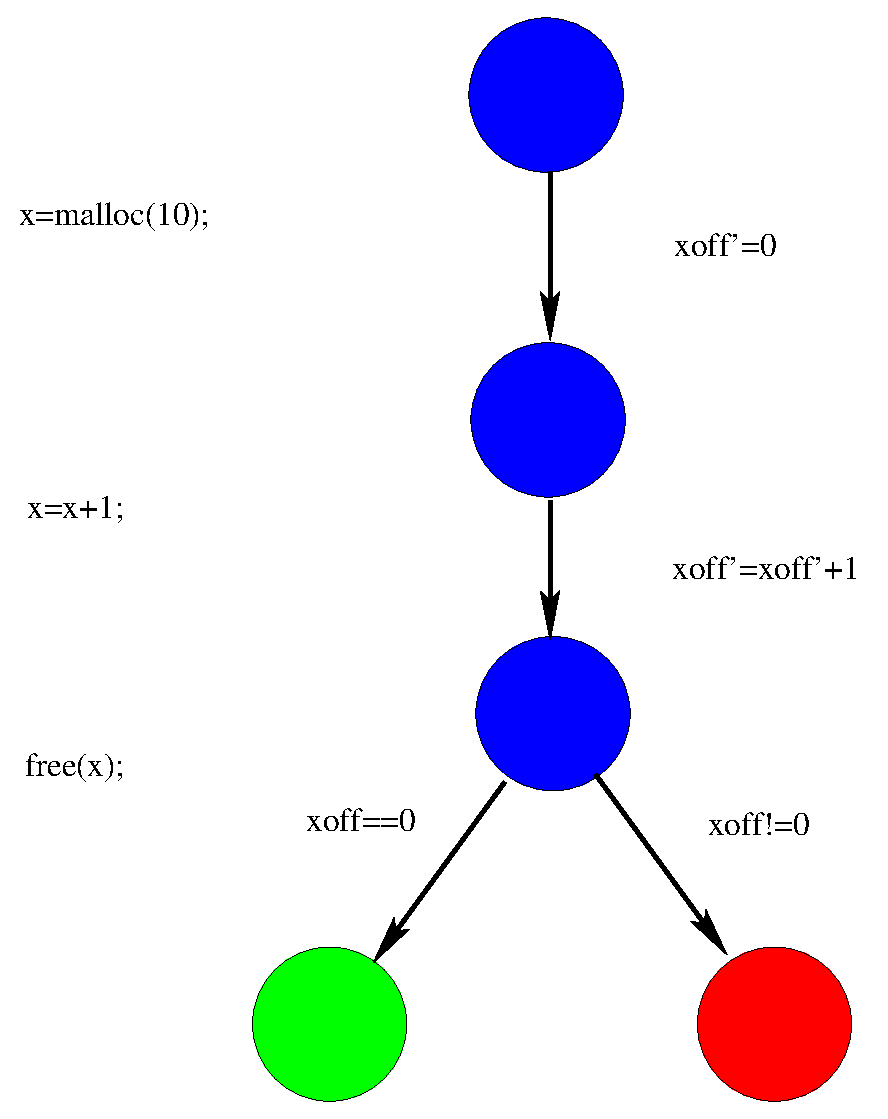
\includegraphics[width=0.4\textwidth]{align.eps}
\end{center}
\end{block}
}



\section{Extracting a SSL+NTS based model using Flata-C}
\begin{frame}
 \frametitle{Outline}
 \tableofcontents[currentsection]
\end{frame}


%\frame{\sectionpage}
%\subsection{The SSL logic : Decribing the Shape}

%\frame{
%\frametitle{Abstract interpretation preliminary part}
% Simple Separation Logic formulae : Abstract domain.

%\begin{block}{Syntax of SSL}
%$$
%\begin{array}{lclr}
%\phi & := & \Formula{\pi}{\sigma} \gspace | \gspace \Exists{l}{\phi} & \mbox{Formulae} \\
%\pi & := & \Pointsto{x}{l} \gspace | \gspace \Pointstonil{x} \gspace | \gspace \EqLoc{l_1}{l_2} \gspace | \gspace \Andpure{\pi_1}{\pi_2} & {\mbox{Pure part}} \\
%\sigma &:=& \Emp  \gspace | \gspace \Alloc{l} \gspace | \gspace \Sep{\sigma_1}{\sigma_2}\ \gspace | \gspace \bot & \mbox{Spatial part}
%\end{array}
%$$
%\end{block}
%}

\subsection{SSL logic to abstract the memory shape}
\frame{
\frametitle{Abstract memory description using SSL}
\begin{block}{SSL describes the following shapes:}
 \begin{itemize}
 \item Relation between stack pointer and location variables
 \item Allocation predicate
 \item Separation operator : Disjoint allocated heap cells
 \end{itemize}
\end{block}
\begin{block}{Properties}
The problems that follow are decidable:
\begin{itemize}
\item Satisfiability (Valid memory configuration)
\item Entailment, Equivalence (Fix point detection)
\item Memory leaks
\end{itemize}
\end{block}

Those problems are solved using rewriting techniques.
}

\subsection{NTL to express arithmetic properties on transitions}
\frame{
\frametitle{Numerical Transition Language }
\begin{block}{Allows express and define:}
\begin{itemize}
 \item Basic types: bool, int, real
 \item Control states: initial, final, error
 \item Transitions: first-order arithemtic
 \item Multi dimesional arrays
 \item Hierarchy: (recursive) function calls
 \item Shared memory concurrency
\end{itemize}

\end{block}

}

\section{What is Flata-C ?}
\begin{frame}
 \frametitle{Outline}
 \tableofcontents[currentsection]
\end{frame}

\subsection{Flata-c is Verification Front-end}

\frame{
\begin{block}{A Verification Front-end}
\begin{itemize} 
\item Takes as input a C Program description using FRAMA-C/Cil AST and CFG.
\item Extracts a NTS base model of the program using static analysis techniques.

 \item 
   \begin{itemize}
   \item Control states having an unsat SSL formula are error states.
   \item Return control states having a sat SSL formula are final.
   \item Entry point of function are initial states.
  \end{itemize}
\item Exports this model in the NTL format
\item The exported model is an over approximation !
 \end{itemize}
\end{block}

\begin{block}{Goal}
\begin{itemize}
\item Query Verification tools for the Reachability of error states.
\item Query Verification tools for the reachability of final states.
\end{itemize}

 Coded as a Frama-C plugin. 
\end{block}
}



%\frame{
%\begin{center}
%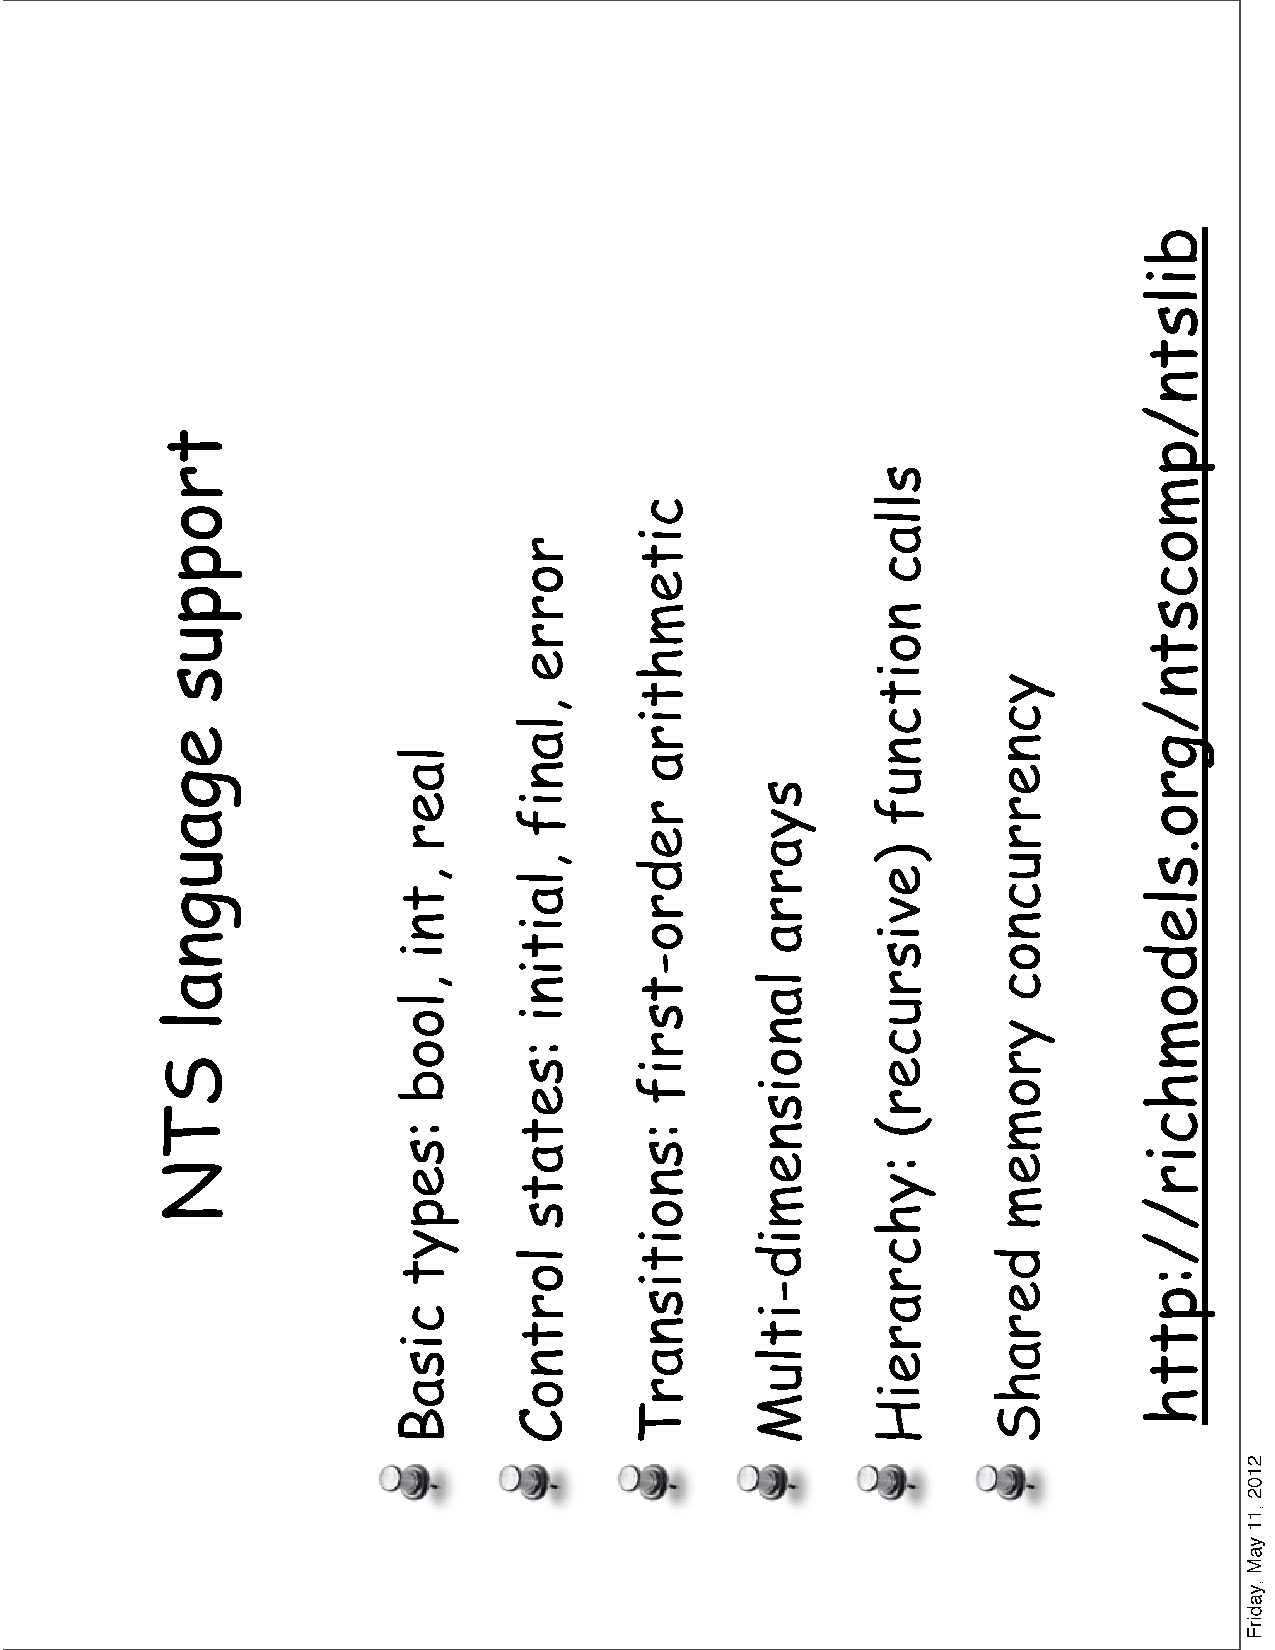
\includegraphics[angle=270,width=0.8\textwidth]{torino-24.pdf}
%\end{center}
%}


%\defverbatim[colored]\lstI{%
%\begin{lstlisting}[language=C,basicstyle=\ttfamily,keywordstyle=\color{red}] 
%void foo(){
% char *x, *y;
% \uncover<1>{Emp}
% x=malloc(10);
% %\uncover<2>{ x-\>l /\ Alloc(l)}
% y=x;
% free(x);
% free(y;)
%}
%\end{lstlisting}
%}



%\begin{frame}{Verifying Heap Consistency}
%\lstI
%\end{frame}






%\frame{
%\frametitle{Tracked property}
%\begin{block}{ Checking that C programs:}
%\begin{itemize}
%\item have no execution run that lead to memory fault,
%\item have no exectution that violates some assertion expressed.
%using arithmetic constraints.
%\end{itemize}
%\tgreen{A verification front-end. }
%\begin{itemize}
%\item Extracts models of C Programs using Abstract Interpretation Techniques. 
%\item Adds \tred{Numerical Transitions Systems} informations on the
%model for \tred{a posteriori Verification Phase}.  
%\item Exports the model into the NTL language.
%\end{itemize}
%\end{block}
%}


%\frame{
%\frametitle{}
%\begin{enumerate}
%\item Extracting an extended cfg from Frama-c cfg $($Cil statements $\times$SSL memory abstractions$)^2$
%\item Labelling the Ecfg transitions with Numerical Transition System expression --Guards, counter affectation and Function Calls.
%\item If a SSL Abs value of a state is $\bot$, define this state as
%an error state.
%\item Export the labelled Ecfg into Nts Format.
%\item Ask an analysis tool --Flata, Eldarica, to check whether 
%some error state is reachable from the entry point (main function).

%\end{enumerate}

%}

\subsection{Flata-c font-end in the  toolchain}
\frame{
\frametitle{Flatac in the tool-chain:}
\begin{center}
\resizebox{9.5cm}{7cm}{\input{toolchain.pstex_t}}
\end{center}

}




%\frame{
%\frametitle{Example of SSL formulae}
%\begin{itemize}
%\item $\Formula{ \Andpure{\Andpure{\Pointsto{x}{l_1}}{\Pointsto{y}{l}}}{\Pointstonil{z}}}{\Emp}$
%\item $\Formula{\Andpure{\Andpure{\Pointsto{x}{l_1}}{\Pointsto{y}{l}}}{\Pointstonil{z}}}{\Alloc{l_1}}$
%\item $\Formula{ \Andpure{\Andpure{\Pointsto{x}{l_1}}{\Pointsto{y}{l}}}{\Pointstonil{z}}}{\Sep{\Alloc{l_1}}{\Alloc{l}}}$
%\item $\Formula{ \Andpure{\Andpure{\Pointsto{x}{l_1}}{\Pointsto{y}{l}}}{\Pointstonil{z}}}{\Sep{\Alloc{l_1}}{\Alloc{l}}}$
%\item $\Formula{ \Andpure{x=y}{\Andpure{\Pointsto{x}{l_1}}{\Pointsto{y}{l}}}}{\Sep{\Alloc{l_1}}{\Alloc{l}}}$ (Unsat)
%\item $\Formula{ \Andpure{x=y}{\Andpure{\Pointsto{x}{l_1}}{\Pointstonil{y}}}}{\Alloc{l_1}}$ (Unsat)
%\item $\Formula{ true }{\Alloc{l}}$ (Leak)
%\end{itemize}
%}
%

%\subsection{Memory model}
%\frame{
%\frametitle{Flata-c Memory model}
%A memory model that associates counters to SSL
%variables :

%\begin{block}{Additional quantitative informations}
%$$
%\begin{array}{lcr}
%\mbox{SSL Variable} & \mbox{NTS counter} & \\
%x\in PVar & \mbox{\texttt{x\_offset}} & \mbox{offset} \\
%l\in LVar & \mbox{\texttt{l\_size}} & \mbox{segment size}
%\end{array}
%$$
%In order to :
%\begin{itemize}
%\item Associate to segment their size.
%\item Associate to pointer their offset.
%\item To express guards on memory access.
%\end{itemize}
%\end{block}
%}



\section{Model extraction}
%\frame{\sectionpage}
\begin{frame}
 \frametitle{Outline}
 \tableofcontents[currentsection]
\end{frame}


\subsection{Cil representation of C programs}
\frame{
\frametitle{Cil representation of C programs}

Cil provides and AST and CFG info from C files.

\begin{block}{Most relevant information}
For each function the AST contains :
\begin{itemize}
\item Variables list : Locals and Formals
\item Return type of the function
\item Statements list 
\item Each Statement has an unique ids $s_{id}$
\item Expressions
\item The CFG provides a successor list for each $s_{id}$
\end{itemize}
\end{block}

}

\frame{
\frametitle{Model extraction : Two main steps}

Input : Cil AST and Control flow graph
Generated Model : Numerical Transition System
  
\begin{block}{ECFG Generation}
\begin{itemize}
\item The vertexes : $(s_{id},\phi)$ where $\phi$ a SSL formula. 
\item The edges are labelled with NTL labels, expressing 
Guards, affectation, and function calls.
\end{itemize}
\end{block}

\begin{block}{ECFG TO NTS compilation}
\begin{itemize}
\item Sort states w.r.t. they are valid, final or erroneous.
\item Pretty print the NTS.
\end{itemize}
\end{block}
}


\frame{
\frametitle{From cil statments to NTS}
\begin{center}
\resizebox{8cm}{!}{\input{Cilstatements.pstex_t}}
\end{center}
}


\subsection{Extraction steps}

\frame{
\frametitle{Step 1 : Compile expression + Valid mem conditions}
\begin{center}
\resizebox{8cm}{!}{\input{compilestep1.pstex_t}}
\end{center}
}

\frame{
\frametitle{Extraction : Basic statement}

\begin{block}{\texttt{Var(v)=expr}}
\begin{center}
\resizebox{8cm}{!}{\input{affectvar.pstex_t}}
\end{center}

\end{block}
}

\frame{
\frametitle{Nts guards for safe memory access}

Let \texttt{x} a $PVar$ such that \texttt{x:}$\tau$\texttt{*}
Let $\texttt{safe\_mem}:\texttt{Cil\_types.expr}\times SSL \mapsto NtsGuards$

\begin{block}{Memory access guards Cil for atomic expressions}
\begin{tabular}{lcl}
Expr &Mem abstraction & Nts Guard \\ 
\texttt{*x} &$\Formula{\Pointsto{x}{l}}{\Alloc{l}}$ & \texttt{true}\\
\texttt{*x} &$\Formula{\Pointsto{x}{l}}{\Emp}$& \texttt{false}\\ 
\texttt{*(x+i)} & $\Formula{\Pointsto{x}{l}}{\Alloc{l}}$& \texttt{v\_i}$\wedge 0\leq i\times$\texttt{sizeof(}$\tau$\texttt{)}$<$\texttt{l\_size}\\
\texttt{tab[i]}&$\Formula{true}{\Emp}$& \texttt{v\_i}$\wedge 0\leq i <$ \texttt{tab\_size}\\
\end{tabular}
\end{block}
}

\frame{
\frametitle{Step 2 : Updating absdomain evaluation}
\begin{center}
\resizebox{8cm}{!}{\input{compilestep2.pstex_t}}
\end{center}
}

\frame{
\frametitle{Extraction : Basic statement}
\begin{block}{\texttt{lval=call(fun,arg1},...,\texttt{argn)}}
Call of \texttt{fun} where \texttt{\{P\} fun \{Q\}}.
\begin{center}
\resizebox{7cm}{!}{\input{funcall.pstex_t}}
\end{center}

\end{block}
}

\frame{
\frametitle{Step 3 : Recurse on all CFG sucessors)}
\begin{center}
\resizebox{8cm}{!}{\input{compilestep3.pstex_t}}
\end{center}
}




%\frame{
%\frametitle{Non deterministic evaluation : validity}
%To any integer variable is associated a validity counter. An
%expression is valid if it is the result of deterministic values.
%\begin{block}{Basic rules}
%\begin{tabular}{lll}
%\texttt{int x;} & \texttt{v\_x = false} \\
%\texttt{int x=cst;} & \texttt{v\_x = true} \\
%\texttt{x=y;} & \texttt{v\_x= v\_y;} \\
%%\texttt{x=ptrw-ptrz;} & \texttt{true} &if $\Formula{\Pointsto{ptrw}{l}\wedge\Pointsto{ptrz}{l}}{.}$\\
%& \texttt{false} &else
%\end{tabular}
%\end{block}

%}




%\frame{
%\frametitle{Control flow statements v.s. basic instructions}

%\begin{block}{Control flow statement}
%One need to consider a transition to $\bot$ guarded by
%$\neg$ \texttt{safe\_mem(expr)}.
%\begin{itemize}
%\item \texttt{if(expr,blockif,blockelse)}
%\item \texttt{switch(expr,case\_list)}
%\end{itemize}
%\end{block}
%Basic statement are easier to model.
%\begin{block}{Instruction statement}
%\begin{itemize}
%\item \texttt{lval=expr}
%\item \texttt{lval=funcall(name,exp list)}
%\end{itemize}
%\end{block}
%}







%\frame{
%\frametitle{Extraction : Basic statment}

%\begin{block}{\texttt{lval=expr}}
%Considered lvals are array element and referenced mem
%cells. 
%\begin{center}
%\resizebox{8cm}{!}{\input{affectlval.pstex_t}}
%\end{center}

%\end{block}
%}





%\frame{
%\frametitle{Extraction : Control Flow operation}
%\begin{block}{\texttt{if(test, stmtif, stmtelse)}}
%Expression \texttt{test} might perform some illegal operations.
%\begin{center}
%\resizebox{5cm}{!}{\input{ifthen.pstex_t}}
%\end{center}
%\end{block}
%}

\frame{
\frametitle{Extraction : Extended Cfg building algorithm}
\begin{block}{Ecfg Generation step}
When generating some $(sid_i,\psi_i)$ from the current abstract
state $(s,\phi)$, using a semantic rule $R$ do:
\begin{itemize}
\item Create a new vertex $(sid_i,\psi_i)$ if $\psi_i$
is the most general formula associated to $sid_i$  or not
entailed by any $(sid_i,\sigma)$.
Create a new edge between the two vertex, with label $R$.
Schedule $(sid_i,\psi_i)$ for futur traversal.
\item Else 
  \begin{itemize}
  \item Add an edge labelled R from the current state 
    to $(sid_i,\psi_g)$ with $\psi_g$ greatest element.
  \end{itemize}
\end{itemize}
\end{block}

}


\subsection{Exporting into NTL format for verification step}

\frame{
\frametitle{Verification Phase : Reachability Analysis}
\begin{block}{Reachability of the error states}
\begin{itemize}
\item Exporting the Ecfg Hierarchical Numerical Transition System.
\item Reachability analysis of the error states by FLATA and/or ELDARICA
\item If some error state is reachable : An alarm is raised.
\item If no error states is reachable : The program is free of the memory fault we consider. 
\end{itemize}
\end{block}
}


%\section{Benchmarks}

%\frame{
%\frametitle{Benchmarks}

%\begin{figure}[h!]
%%\begin{scriptsize}
%{\small
%\begin{minipage}[t]{.5\textwidth}
%%\begin{scriptsize}
%\begin{tabular}[t]{lrrrr}
%\hline
%%\multirow{2}{*}{Model} & \multicolumn{2}{c}{ Time [s]} \\
%& F. & E. & S. & D. \\
%\hline
%\multicolumn{3}{l}{\textbf{(a) Examples from TACASO6\[\]}} \\
%\hline
%anubhav (C)  &  0.6  & 1.5 &  1.8  &  1.5\\
%copy1 (E)  &  1.7 & 8.1  &  1.2  &  3.5\\
%cousot (C) &  0.5 & -  &  -  &  4.3 \\
%loop1 (C) &  0.4 & 2.1  &  0.9  &  2.1 \\
%loop (C) &  0.4 & 0.3  &  0.9  &  0.3 \\
%scan  (E) &  2.4 & -  &  1.0  &  2.9 \\
%string\_concat1  (E) &  4.4  & -  &  3.2  &  5.0  \\
%string\_concat  (E) &  4.1  & -  &  2.5  &  4.2  \\
%string\_copy  (E) &  3.7  & -  &  1.5  &  3.6  \\
%substring1 (E) &  0.3  & 1.6  &  23.9  &  1.5 \\
%substring (E) &  1.8  & 0.6  &  1.6  &  0.6 \\
%\hline
%\end{tabular}
%\end{minipage}%
%\hspace*{-2ex}%
%} % end small
%\end{scriptsize}
%\end{figure}
%\textbf{F}lata, \textbf{E}ldarica, Eldarica (\textbf{S}tatic loop acceleration)
% and CEGAAR (\textbf{D}ynamic acceleration).  

%}

\section{Development and Current State of Flata-c}

\begin{frame}
 \frametitle{Outline}
 \tableofcontents[currentsection]
\end{frame}


\frame{
\frametitle{Flata-c currently support}
\begin{block}{Currently implemented}
  \begin{itemize}
    \item Assert checking on first order arithmetic. 
    \item Function calls with scalar values and pointers.
    \item Inner function memory model extraction.
    \item NTL code generation.
  \end{itemize}
\end{block}
}


\frame{
\frametitle{Current development}
\begin{block}{Current development}
  \begin{itemize}
  \item Handling arbitrary parameters in function calls.
  \item Hoar logic style pre and post condition inference.
  \item Better handling of Non-determinism.
  \item Counter-example trace analysis.
  \end{itemize}
\end{block}
}


\section{Personal contributions}
\begin{frame}
 \frametitle{Outline}
 \tableofcontents[currentsection]
\end{frame}


\frame{
  \begin{block}{Others and Collaborative contributions}
    \begin{itemize}
      \item SSL logic : Radu Iosif
      \item NTL : Radu Iosif, Viktor Kuncak(EPFL), Vojnar Tomas( Brno University) 
      \item Verification tools : Flata (Filip Konecny) and Eldarica (Hossein Hojjat)
    \end{itemize}
  \end{block}

  \begin{block}{Personal Contributions}
    \begin{itemize}
    \item Designed and Implementation of decision procedures. 
      (OCaml SSL library)
    \item Ocaml implementation of the NTL library as a
      target language.
    \item Designed and implemented the components of
      the model extraction front-end.
    \end{itemize}
\end{block}
}


\section{Introspective Analysis}
\frame{\sectionpage}

\frame{
  \begin{block}{}
    \begin{itemize}
      \item Incrementally adding features led to some design inconsistencies
      \item The semantic action module is not suited for specification
        inference.
      \item Need to design a language for expressing SSL+NTL Hoar like 
        specifications for functions.
      \item Choosing an Object oriented design for the static analyser
        part proved too be a poor choice as it makes code hard to read
        and brings nothing as counterpart.
      \item Both SSL and NTL implementation have been externalized as
        separated libraries, in order to make code maintenance and
        featured adding, as well as unitary testing easier.
      \item I will try to devise better strategies to maintain two
        branches of the same software when urgent deadline are looming.
      \item Not casually evaluating how long it takes to achieve a task.
      \end{itemize}
  \end{block}

}



\section{Why my application for a C/C++ Compiler Developer position at The Mathworks ?}

\begin{frame}
 \frametitle{Outline}
 \tableofcontents[currentsection]
\end{frame}

\frame{
\frametitle{Why my application for a C/C++ Compiler Developer position at The Mathworks ?}
\begin{block}{Main motivations}
  \begin{itemize}
    \item Good opportunity to put my skills at use and to the test
    \item I'm looking for working together with skilled and communicating colleagues.
    \item A Great opportunity to gain outstanding skills in the field of compilation
    \item I expect to work on ambitious and challenging projects 
    \item I would be proud of bringing a contribution to famous softwares
    \item The Mathworks offers an international working environment
  \end{itemize}
\end{block}
}
%\frame{
%\frametitle{Benchmarks}

%\begin{figure}[h!]
%\begin{scriptsize}
%{\small
%\begin{minipage}[t]{.5\textwidth}
%\begin{scriptsize}
%\begin{tabular}[t]{lrrrr}
%\hline
%%\multirow{2}{*}{Model} & \multicolumn{2}{c}{ Time [s]} \\
%& F. & E. & S. & D. \\
%\hline
%\multicolumn{3}{l}{\textbf{ Examples from Monniaux}} \\
%boustrophedon (C) &  -  & -  &  -  &  12.2 \\
%gopan (C) &  0.5  & -  &  -  &  6.7 \\
%halbwachs (C) & -  & -  &  1.6  &  8.2 \\
%rate\_limiter (C) &  -  & 7.2  &  2.7  &  7.1 \\
%\hline
%\multicolumn{3}{l}{\textbf{(e) NECLA benchmarks}} \\
%\hline
%inf1 (E) &  0.1  & 0.3  &  0.3  &  0.3 \\
%inf4 (E) &  0.8  & 0.5  &  0.5  &  0.5 \\
%inf6 (C) & 0.1  & 0.3  &  0.3  &  0.3 \\
%inf8 (C) &  0.3  & 0.6  &  0.6  &  0.6 \\
%\hline
%\end{tabular}
%\end{minipage}%
%\hspace*{-2ex}%
%} % end small
%%\end{scriptsize}
%\end{figure}
%\textbf{F}lata, \textbf{E}ldarica, Eldarica (\textbf{S}tatic loop acceleration)
 %and CEGAAR (\textbf{D}ynamic acceleration).  

%}


%\fram
%\frame{
%\frametitle{How to label terms with A.P. ?}
%\begin{center}
%\resizebox{10cm}{!}{\input{LabelLucas.pstex_t}}
%\end{center}
%}
%
%\frame{
%\frametitle{Precision of computational sets}
%\begin{center}
%\resizebox{8cm}{!}{\input{Precision.pstex_t}}
%\end{center}
%}
%

\end{document}

\frame{
\frametitle{Example}
$$
\begin{array}{lll}
\mbox{C "statement"} & \mbox{SSL formula}& \texttt{NTS transition} \\
\mbox{\texttt{int *x;}} &\Formula{\exists l \Pointsto{x}{l}}{\Emp}&\texttt{offset\_x'=0}\\
\mbox{\texttt{x=malloc(10);}} &\Formula{\exists l \Pointsto{x}{l}}{\Alloc{l}}&\texttt{size\_l=10}\\
\mbox{\texttt{x++;}} & \Formula{\exists l \Pointsto{x}{l}}{\Alloc{l}}& \texttt{offset\_x'+=sizeof(int)} \\
\mbox{\texttt{int y =*x;}} & \Formula{\exists l \Pointsto{x}{l}}{\Alloc{l}}& \texttt{offset\_x'} < \mbox{size\_l} \\
&\Formula{\exists . l \Pointsto{x}{l}}{\Alloc{l}}& \mbox{havoc(y)}
\end{array}
$$

}

\frame{
\frametitle{Example}
$$
\begin{array}{lll}
\mbox{C "statement"} & \mbox{SSL formula}& \texttt{NTS transition} \\
\mbox{\texttt{int *x;}} &\Formula{\exists l \Pointsto{x}{l}}{\Emp}&\texttt{offset\_x'=0}\\
\mbox{\texttt{x=malloc(10);}} &\Formula{\exists l \Pointsto{x}{l}}{\Alloc{l}}&\texttt{size\_l=10}\\
\mbox{\texttt{x++;}} & \Formula{\exists l \Pointsto{x}{l}}{\Alloc{l}}& \texttt{offset\_x'+=sizeof(int)} \\
\mbox{\texttt{int y =*x;}} & \Formula{\exists l \Pointsto{x}{l}}{\Alloc{l}}& \texttt{offset\_x'}<\mbox{size\_l} \\
&\Formula{\exists . l \Pointsto{x}{l}}{\Alloc{l}}& \mbox{havoc(y)}\\
\mbox{\texttt{x+=10;}} & \Formula{\exists l \Pointsto{x}{l}}{\Alloc{l}}& \texttt{offset\_x'+=10*sizeof(int)} \\
\end{array}
$$
}



\frame{
\frametitle{Example}
$$
\begin{array}{lll}
\mbox{C "statement"} & \mbox{SSL formula}& \texttt{NTS transition} \\
\mbox{\texttt{int *x;}} &\Formula{\exists l \Pointsto{x}{l}}{\Emp}&\texttt{offset\_x'=0}\\
\mbox{\texttt{x=malloc(10);}} &\Formula{\exists l \Pointsto{x}{l}}{\Alloc{l}}&\texttt{size\_l=10}\\
\mbox{\texttt{x++;}} & \Formula{\exists l \Pointsto{x}{l}}{\Alloc{l}}& \texttt{offset\_x'+=sizeof(int)} \\
\mbox{\texttt{int y =*x;}} & \Formula{\exists l \Pointsto{x}{l}}{\Alloc{l}}& \texttt{offset\_x'}<\mbox{size\_l} \\
&\Formula{\exists . l \Pointsto{x}{l}}{\Alloc{l}}& \mbox{havoc(y)}\\
\mbox{\texttt{x+=10;}} & \Formula{\exists l \Pointsto{x}{l}}{\Alloc{l}}& \texttt{offset\_x'+=10*sizeof(int)} \\
\mbox{\texttt{*x=42;}} & \bot & \tred{\texttt{offset\_x}\geq\mbox{size\_l}} \\
\end{array}
$$

\tred{Access to \texttt{*x} is out of bounds of allocated segment at \texttt{l}.}
}


\frame{
\frametitle{Compiling expressions}


\begin{block}{From pointer arithmetic to Nts expressions}
$$
\begin{array}{|lll|}
\hline
\base{\phi}{x}&:=& l \mbox{ if }  \Pointsto{x}{l} \in \Pp{\phi} \\
\base{\phi}{\NULL} &:=& \nil \gspace \forall \phi \\
\base{\phi}{P+I} &:=& \base{\phi}{P} \\

%\end{array}
%$$


%}

%\frame{
%\frametitle{Compiling Integer expressions}

%$$
%\begin{array}{|lll|}
 \interpa{\phi}{n} & := & n \\
\interpa{\phi}{i} & := & \icnt{i} \\
\interpa{\phi}{\NULL} & := & 0 \\
\interpa{\phi}{x} &:=& \ptroffset{x} \\
\interpa{\phi}{x_1 - x_2} & :=&  \ptroffset{x_1}-\ptroffset{x_2} \\
\interpa{\phi}{P+I} & := & \interpa{\phi}{P}+\interpa{\phi}{I}\times \sizeof{\tau}, \mbox{ where } P:\tau *\\
\interpa{\phi}{P_1 - P_2} & := & ( \interpa{\phi}{P_1}-\interpa{\phi}{P_2}) / \sizeof{\tau}, \mbox{ where } P_1:\tau * \\
\interpa{\phi}{I_1+I_2} &:=& \interpa{\phi}{I_1} + \interpa{\phi}{I_2} \\
\interpa{\phi}{I_1 \times I_2} &:= &\interpa{\phi}{I_1} \times \interpa{\phi}{I_2} \\
\hline
\end{array}
$$
\end{block}
}


\frame{
\frametitle{Compiling booleans to Nts guards}

\begin{block}{}
$$
\begin{array}{lll}

\interpa{\phi}{P_1 == P_2} &:=& \left \lbrace \begin{array}{ll} 
        \interpa{\phi}{P_1} == \interpa{\phi}{P_2} & \mbox{ if } \base{\phi}{P_1}\seq\base{\phi}{P_2} \\
        \bot & \mbox{else} 
        \end{array} \right . \\
&&\\
\interpa{\phi}{P_1 != P_2} &:=& \left \lbrace \begin{array}{ll} 
        \interpa{\phi}{P_1} != \interpa{\phi}{P_2} & \mbox{ if } \base{\phi}{P_1}\seq\base{\phi}{P_2} \\
        \bot & \mbox{else} 
        \end{array} \right . \\
&&\\
\interpa{\phi}{P_1 \bowtie P_2} &:=& \left \lbrace \begin{array}{ll} 
        \interpa{\phi}{P_1} \bowtie \interpa{\phi}{P_2} & \mbox{ if } \base{\phi}{P_1}\seq\base{\phi}{P_2} \\
        \bot & \mbox{else} 
        \end{array} \right . \\ 
\end{array}
$$
\end{block}
}


\frame{
\frametitle{Compiling expressions}


\begin{block}{From pointer arithmetics to Nts expressions}
$$
\begin{array}{|lll|}
\hline
\base{\phi}{x}&:=& l \mbox{ if }  \Pointsto{x}{l} \in \Pp{\phi} \\
\base{\phi}{\NULL} &:=& \nil \gspace \forall \phi \\
\base{\phi}{P+I} &:=& \base{\phi}{P} \\

%\end{array}
%$$


%}

%\frame{
%\frametitle{Compiling Integer expressions}

%$$
%\begin{array}{|lll|}
 \interpa{\phi}{n} & := & n \\
\interpa{\phi}{i} & := & \icnt{i} \\
\interpa{\phi}{\NULL} & := & 0 \\
\interpa{\phi}{x} &:=& \ptroffset{x} \\
\interpa{\phi}{x_1 - x_2} & :=&  \ptroffset{x_1}-\ptroffset{x_2} \\
\interpa{\phi}{P+I} & := & \interpa{\phi}{P}+\interpa{\phi}{I}\times \sizeof{\tau}, \mbox{ where } P:\tau *\\
\interpa{\phi}{P_1 - P_2} & := & ( \interpa{\phi}{P_1}-\interpa{\phi}{P_2}) / \sizeof{\tau}, \mbox{ where } P_1:\tau * \\
\interpa{\phi}{I_1+I_2} &:=& \interpa{\phi}{I_1} + \interpa{\phi}{I_2} \\
\interpa{\phi}{I_1 \times I_2} &:= &\interpa{\phi}{I_1} \times \interpa{\phi}{I
_2} \\
\hline
\end{array}
$$
\end{block}
}


\frame{
\frametitle{Compiling booleans to Nts guards}

\begin{block}{}
$$
\begin{array}{lll}

\interpa{\phi}{P_1 == P_2} &:=& \left \lbrace \begin{array}{ll} 
        \interpa{\phi}{P_1} == \interpa{\phi}{P_2} & \mbox{ if } \base{\phi}{P_1}\seq\base{\phi}{P_2} \\
        \bot & \mbox{else} 
        \end{array} \right . \\
&&\\
\interpa{\phi}{P_1 != P_2} &:=& \left \lbrace \begin{array}{ll} 
        \interpa{\phi}{P_1} != \interpa{\phi}{P_2} & \mbox{ if } \base{\phi}{P_1}\seq\base{\phi}{P_2} \\
        \bot & \mbox{else} 
        \end{array} \right . \\
&&\\
\interpa{\phi}{P_1 \bowtie P_2} &:=& \left \lbrace \begin{array}{ll} 
        \interpa{\phi}{P_1} \bowtie \interpa{\phi}{P_2} & \mbox{ if } \base{\phi}{P_1}\seq\base{\phi}{P_2} \\
        \bot & \mbox{else} 
        \end{array} \right . \\ 
\end{array}
$$
\end{block}
}

\frame{
\frametitle{Extraction : Extended Cfg building algorithm}

\begin{itemize}
\item If $\exists (sid,\psi)\in S$ s.t. $sid=s_{next}$ and $\psi\vdash\phi$
then $\to = \to \cup (s_{curr},\phi),R,(s_{next},\psi)$
\item Else 
  \begin{itemize}
  \item $\to = \to \cup (s_{curr},\phi),R,(s_{next},\phi^{\prime})$
  \item Recurse on abstract state $(s_{next},\phi^{\prime})$
  \end{itemize}
\end{itemize}

\begin{block}{Termination}
This algorithm terminates as the $sid$ index is a fixed set and
that the SSL formula w.r.t. the partial order $\vdash$ is a 
complete lattice.
\end{block}
}


\frame{
\frametitle{Nts guards for safe memory access}
\begin{block}{Cil expression type definition (Non exhaustive)}
\begin{tabular}{l}
\texttt{UnOp(UOp,expr)} \\
\texttt{BinOp(BOp,expg,expd)}\\
\texttt{UOP}=\texttt{UnMin| BNot | Neg}$\ldots$ \\
\texttt{BOP}=\texttt{BAnd|BOr}$\ldots$\\
\phantom{UOP}\texttt{Plus|Minus|Prod|Div}$\ldots$\\
\phantom{BOP}\texttt{PlusPI|MinusPI|MinusPP}$\ldots$\\
\end{tabular}
\end{block}

\begin{block}{\texttt{valid\_mem} of Cil expression}
\begin{tabular}{ll}
Cil expr & \texttt{valid\_mem} \\
\texttt{UnOp(UOp,expr)} & \texttt{valid\_mem(expr)}\\
\texttt{BinOp(BOp,expg,expd)} & \texttt{valid\_mem(expg)}$\wedge$\texttt{valid\_mem(expg)} \\
\end{tabular}
\end{block}
}



%\frame{
%\frametitle{Exporting the ECFG of a function into the NTL format}
%\begin{itemize}
%\item Assign to all $(sid,\phi)\in S$ an unique id $id_{sid,\phi}$.
%\item Input state $IdS_i=\{id_{s_0,\phi_{enty}}\}$.
%\item Error states : $IdS_{err}=\lbrace id_{s,\phi} | \phi = \bot \rbrace$.
%\item States : $IdS = \lbrace id_{s,\phi} | (s,\phi) \not\in(S_i \cup S_f \cup S_{err})\rbrace$
%\item Transitions : 
%  \begin{itemize}
%  \item For all $\tred{(s,\phi)}\times R \tgreen{(q,\psi)} \in \to$ do :
%  \item Print $\tred{id_{s,\phi}}\to\tgreen{id_{q,\psi}} \{R\}$
% \end{itemize}
%\end{itemize}



%}
